\documentclass{article}

%% Page Margins %%
\usepackage{geometry}
\geometry{
    top = 0.75in,
    bottom = 0.75in,
    right = 0.75in,
    left = 0.75in,
}

\usepackage{amsmath}
\usepackage{graphicx}
\usepackage{parskip}

\title{Project Report}

\author{ZENG ZIXUAN 1008533419}

\begin{document}
\maketitle

\section{Demonstration 1: Milestone 1/2/3}
\begin{enumerate}
\item Decide on what will be, and how it will be stored and laid out, in memory. \\ \\
My design of bitmap is 258$\times$512, with a 1$\times$1 unit pixel. So the ADDR\_DSPL which started out at 0x10008000 overflowed to 0x10088000. Therefore I added .space 491520 at the beginning of .data section to prevent my data from being overwritten.\\\\
There are 3 labels in the immutable .data section.\\
ADDR\_DSPL: For projecting colours onto bitmap display with memory address 0x10008000.\\
ADDR\_KBRD: For accessing keyboard inputs with memory address 0xffff0000.\\
MY\_COLOURS: For storing all my colours: 0x00ff0000(red), 0x0000ff00(green), 0x000000ff(blue), ect.\\ \\
There are 3 labels in the mutable .data section.\\
BRICKS: .space 600. For storing coordinates x, y and values of lives for all 50 bricks over 5 rows (200*3).\\
PADDLE: .space 4. For storing location of the paddle.\\
BALL: .space 16. For storing coordinates x, y and momentum x, y of ball.\\
LIVES: .space 4. For storing player's remaining attempts.\\\\

\item Include a screenshot (or multiple screenshots) of memory demonstrating that it has been laid out according to your plan.
\begin{figure}[ht!]
    \centering
    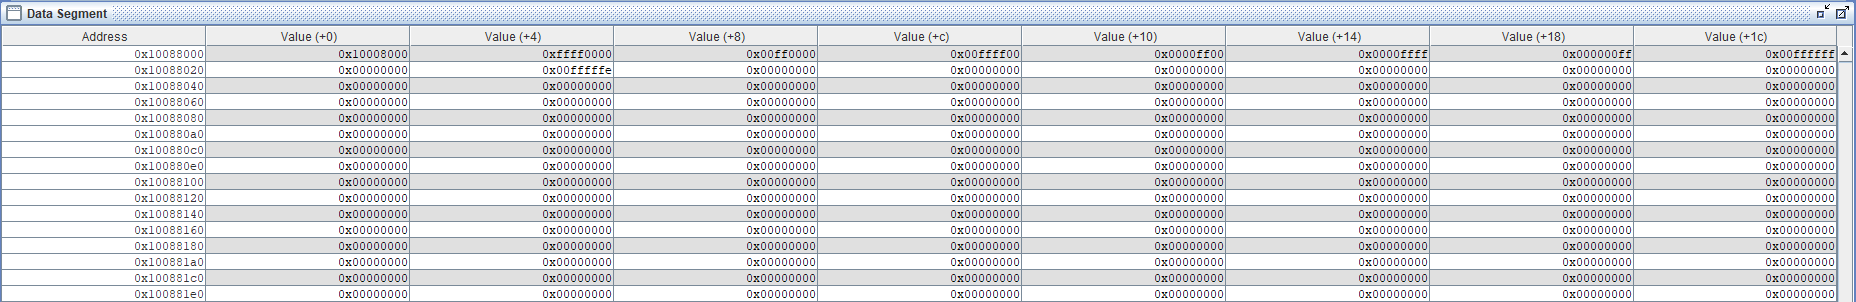
\includegraphics[width=1\textwidth]{1.png}
    \caption{A screenshot of .data.}
    \label{f:.data}
\end{figure}

\pagebreak
\item Include a screenshot of the static scene in your report.
\begin{figure}[ht!]
    \centering
    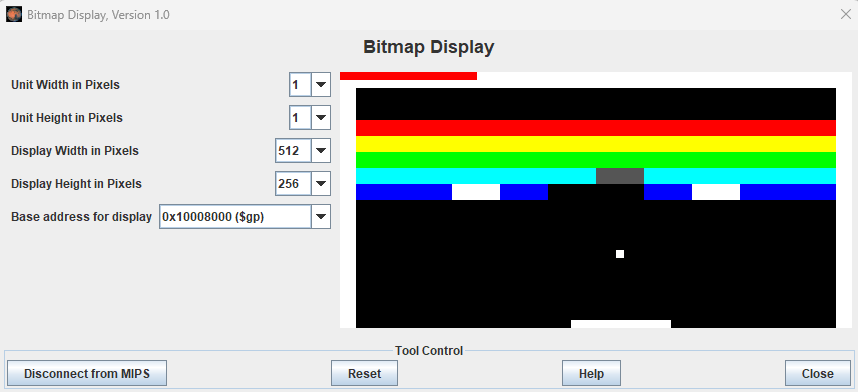
\includegraphics[width=1\textwidth]{2.png}
    \caption{A screenshot of scene in progress.}
    \label{f:.data}
\end{figure}
\\
\item How will the ball change directions when it collides?\\ \\
When it collides with a horizontal surface, the x momentum of the ball should remain the same while the y momentum flips to its additive inverse.\\
When it collides with a vertical surface, the y momentum of the ball should remain the same while the x momentum flips to its additive inverse.\\
However, when the ball hits my paddle, x and y momentum of the ball will be reset towards a new direction based on which part of the paddle it hit.\\
\end{enumerate}


\section{Demonstration 2: Milestone 4/5}
\begin{enumerate}
\item I finished 5 easy features and 1 hard feature:\\\\
Easy:\\
1. Support “multiple lives” (at least 3) so that the player can attempt to make all the bricks disappear multiple times. The state of previous attempts (i.e., broken bricks) should be retained forsubsequent attempts.\\
3. Support different speeds for the ball. That is, on collisions, the ball not only changes direction by also changes speed.\\
5. Allow the user to pause the game by pressing the keyboard key p.\\
6. Add a time limit to the game.\\
7. Add ‘unbreakable’ bricks\\\\
Hard:\\
3. Require bricks be hit by the ball multiple times before breaking. Demonstrate the players progress toward breaking a brick in some way (e.g., different colours).\\
\end{enumerate}

\section{How to Play}
\begin{enumerate}
\item Set up bitmap display configuration accordingly, assemble and run.
\item Ball automatically fires upwards from the paddle located at the bottom center. After hitting an object, the ball will bounce with a different velocity.
\item Press or hold key A or D to move the paddle left or right to catch the ball. If the ball hits the center of the paddle, it will bounce upwards. If the ball hits the left part of the paddle, it will bounce left with different angles depending on how far left it is hitting the paddle. Same goes for the right.
\item There will be two white blocks of unbreakable wall within five layers of bricks, try not to target them. Also, all bricks have two lives. On first hit, it will turn grey. On second hit, the brick will break and dissapear.
\item You will have three attempts in total. If you drop the ball less than three times, press R for another attempt. If you lose three lives, the game is over.
\item During the game, you can pause at any time by pressing P. If you want to resume the game, press R. Also, if you want to quit the game, press Q at any time.
\item There is a time bar at the top of the screen. When it hits the right edge, your time is up and you have failed one attempt.
\item Lastly, have fun!
 
\end{enumerate}



\end{document}